\section{实验一：起点状态（子主张 S1）}\label{sec:s1}

本章逐组给出起点状态的消融结果（总览见图 \ref{fig:ablation}），回答 S1 的两个成立条件：
\textbf{热启动是否显著优于空白}（\S\ref{sec:a1}）与\textbf{写入是否显著优于 $\mathit{lock}$}（\S\ref{sec:a2}），
再用跨文档边界（\S\ref{sec:a3}）与组件级归因（\S\ref{sec:s1-attr}）回答「信息由谁承载」。

\begin{figure}[H]
\centering
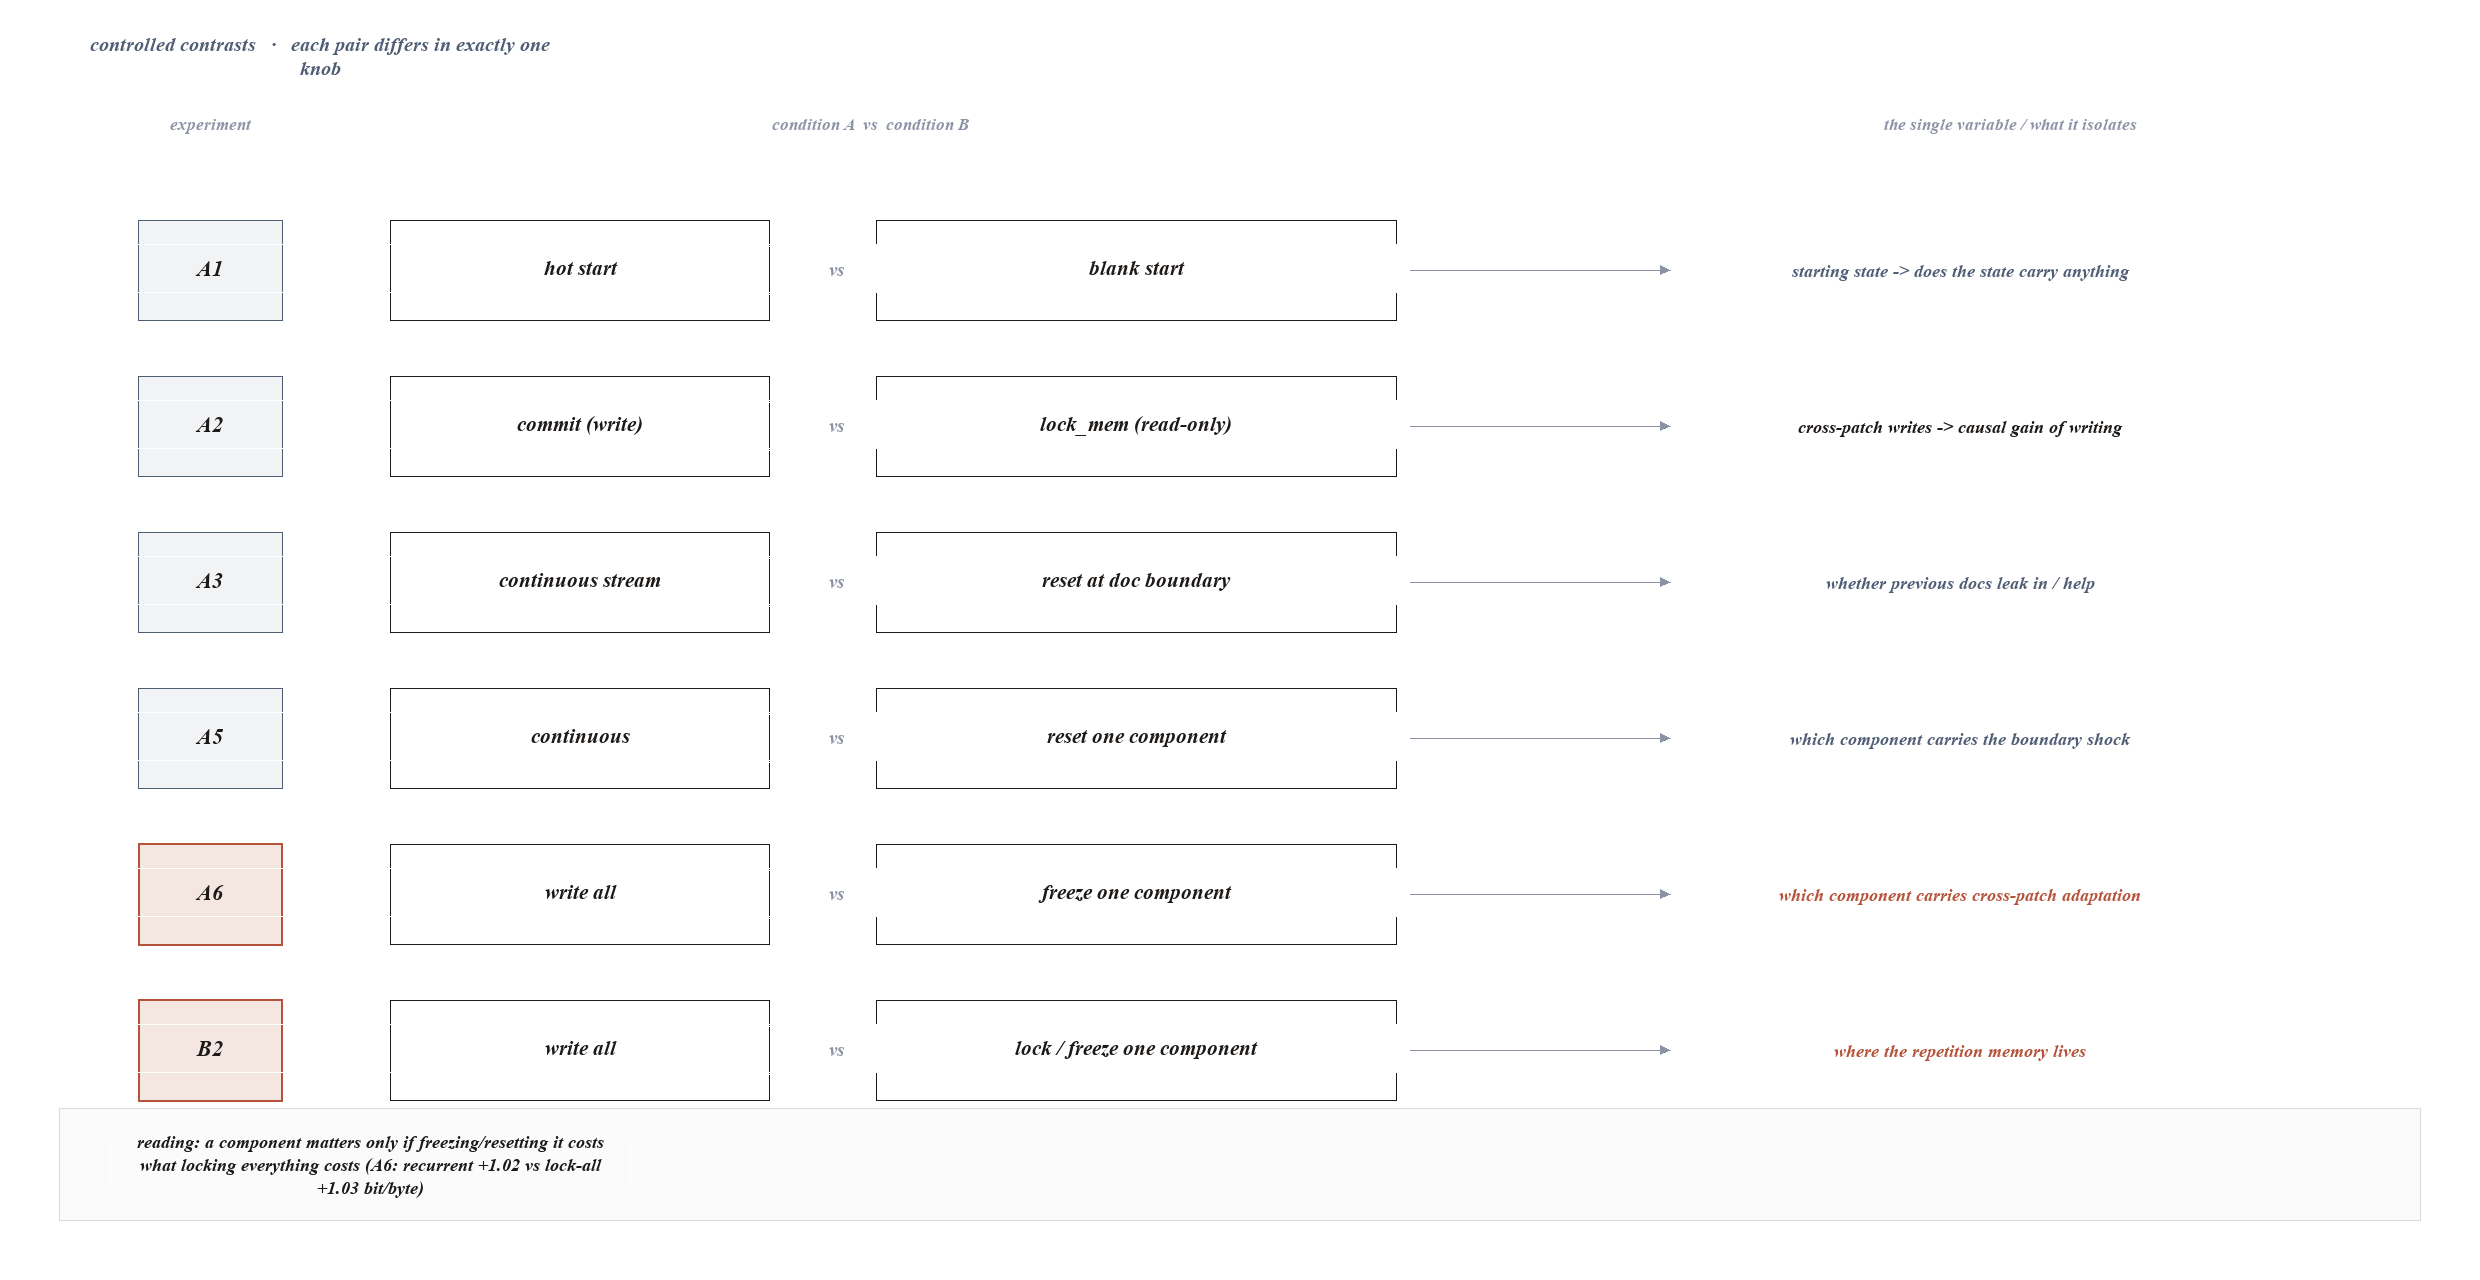
\includegraphics[width=\linewidth]{fig_ablation_matrix.png}
\caption{受控对照一览（Visio 绘制，源文件 \texttt{figs/fig\_ablation\_matrix.vsdx}）。
每一对条件只差一个旋钮；右侧一列写出该对照隔离出的变量。
阅读方式写在图底：一个分量只有在「冻结/重置它的代价等于冻结全部写入的代价」时，才算真正承载了这门功能。}
\label{fig:ablation}
\end{figure}

\subsection{热启动 vs 空白起步（A1）}\label{sec:a1}

\textbf{设计。}同一份文本、同一前向协议，唯一变量是初始状态：
热启动（\texttt{load\_model\_checkpoint} 取训练稳态快照）对空白
（\texttt{init\_inference\_state}：恒等 memory $+$ 零 recurrent/queue/MTM）。
\textbf{计分窗口对齐}：三个「空白 $+$ 预热 $W$ token」档（$W\in\{0,256,1024\}$）在实现上只是
「从第 $W/64$ 个 patch 起计分」——每个 patch 都会被前向，所以三档的状态轨迹完全相同。
既然状态轨迹相同，三档就必须在\textbf{同一个计分窗口}上比较，否则「预热」只是个伪变量。
本文按此对齐：所有条件一律从第 16 个 patch 起计分。

\textbf{结果（表 \ref{tab:a1}、图 \ref{fig:a1}）。}对齐窗口（48 个 patch $=$ 3\,KB，文本取自 sft 尾部 4097 字节）：
热启动 $1.588\bits$，空白 $5.319\bits$，差距 $\mathbf{3.731\bits}$。
三个空白档在对齐窗口上的数值\textbf{逐位相同}（最大差 $0.000\mathrm{e}{+}0$）——这直接印证了
「预热档是伪变量」。窗口内\textbf{无追平趋势}（图 \ref{fig:a1} 右：$blank-hot$ 全程在 $1.1$--$4.6\ \nats$ 之间波动，无下行）。

若不做窗口对齐（即照早期报告的写法），三档分别是 $5.668/5.544/5.319\bits$，
其中「$0.35$ bits 的挽回」全部来自把最差的头几个 patch 排除在计分之外，
而不是模型写得慢——这一点必须在论文里写清，否则会误读成「空白态可以通过预热追上」。

% A1：热启动 vs 空白起步（对齐计分窗口）
\begin{table}[t]
\centering
\caption{A1 热启动 vs 空白起步。文本为 \texttt{sft.jsonl} 尾部 4097 字节（跨域、零污染），
所有条件记分窗口相同（第 16--63 个 patch，共 48 个 patch $=$ 3\,KB）。
「预热」档在对齐窗口上数值逐位相同（最大差 $0.000\mathrm{e}{+}0$），故不是有效变量；
最后一行给出未对齐窗口时的数值，两者相差的 $0.35\bits$ 纯属窗口效应。}
\label{tab:a1}
\small
\begin{tabular}{@{}lccc@{}}
\toprule
条件 & 起点状态 & 计分窗口 & bits/byte \\
\midrule
热启动（hot） & 训练稳态快照 & 48 patch（对齐） & $\mathbf{1.588}$ \\
空白（blank） & 恒等 memory $+$ 零其余 & 48 patch（对齐） & $5.319$ \\
空白 $+$ 预热 256 & 同上（同一轨迹） & 48 patch（对齐） & $5.319$ \\
空白 $+$ 预热 1024 & 同上（同一轨迹） & 48 patch（对齐） & $5.319$ \\
\midrule
\multicolumn{2}{@{}l}{热启动 $-$ 空白（对齐窗口）} & 48 patch & $\mathbf{+3.731}$ \\
\midrule
热启动（未对齐） & 训练稳态快照 & 64 patch & $1.623$ \\
空白 $+$ 预热 0（未对齐） & 恒等 memory $+$ 零其余 & 64 patch & $5.668$ \\
空白 $+$ 预热 256（未对齐） & 同上 & 60 patch & $5.544$ \\
\bottomrule
\end{tabular}
\end{table}


\begin{figure}[t]
\centering
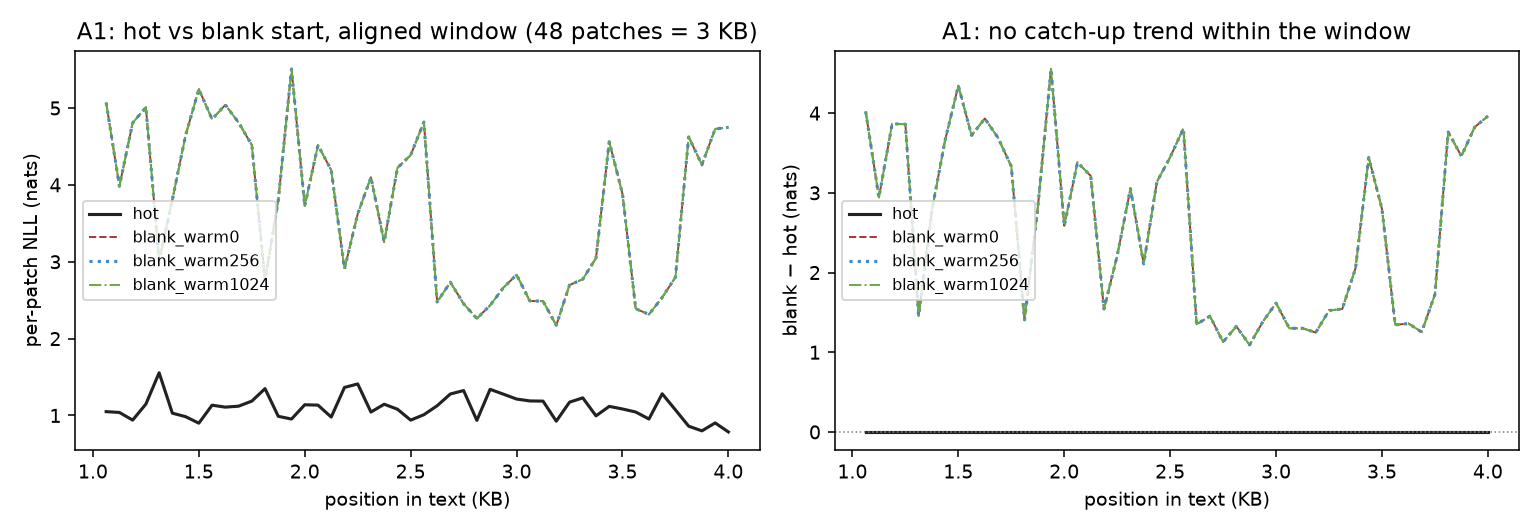
\includegraphics[width=\linewidth]{fig_a1_hot_vs_blank.png}
\caption{A1：热启动 vs 空白起步（同一计分窗口，48 个 patch $=$ 3\,KB）。
左：逐 patch NLL；三条空白曲线\textbf{完全重合}（预热档同一计算），热启动全程低 $1$--$4\ \nats$。
右：$blank-hot$ 的差值曲线，窗口内无收敛趋势。}
\label{fig:a1}
\end{figure}

\textbf{判定。}S1 的第一条成立：热启动显著优于空白，且差距不是「写入速度」能解释的
（对齐窗口内空白没有变小趋势）。
\textbf{推论与限定}：空白态的差是结构性的——恒等/零状态使 delta 规则的读写链路偏离训练操作点，
前向通道在空白态下并未进入正常工作区。因此空白\textbf{不能}作为「无记忆」的干净对照，
只能作为「状态贡献」的上界演示；热启动记忆的成分分解（通用先验 / 同分布偏向 / 逐样本痕迹）
见 \S\ref{sec:dline}。

\subsection{写入的因果贡献：$\mathit{lock}$ 对照（A2）}\label{sec:a2}

\textbf{设计。}同一份同分布 held-out（16\,KB，seed $\in\{0,1,2\}$ 三份不同文本），
两个条件：\texttt{write}（正常 commit）与 \texttt{lock}（$\mathit{lock\_mem}=\mathrm{true}$，
跨 patch 持久写入关闭）。由于 $\mathit{lock}$ 不改变首个 patch 的输出（\S\ref{sec:model-io}），
两条件在前 64 字节逐位一致，差异只来自「从第二个 patch 起，这段上下文是否被写进状态」。
指标为 bits/byte，并按 seed 成对求差（\S\ref{sec:stats}）。

\textbf{结果（表 \ref{tab:a2}、图 \ref{fig:a2}）。}
$\mathrm{write}=1.581\pm0.493$、$\mathrm{lock}=2.580\pm0.399\bits$，
\textbf{成对差值 $=+0.999\pm0.095\bits$}（三份文本分别为 $0.978/1.091/0.927$）。
逐 patch 看，差值\textbf{随后段增长}：前 32 个 patch $+0.585\nats$、后 32 个 patch $+0.771\nats$——
写入的收益是\textbf{累积}的。

% A2：写入 vs 只读（lock）
\begin{table}[t]
\centering
\caption{A2 写入 vs 只读（$\mathit{lock\_mem}$）。同分布零污染 held-out 16\,KB，
三个 seed 为三份不同文本。主报\textbf{成对差值}（先算每份文本的差再平均），
它剔除了文本难度差异；末两行为 seed 0 的逐 patch 差值演化，显示写入收益随上下文累积。}
\label{tab:a2}
\small
\begin{tabular}{@{}lccc@{}}
\toprule
seed（文本） & write (bits/byte) & lock (bits/byte) & 差值（lock $-$ write） \\
\midrule
0 & $1.661$ & $2.639$ & $+0.978$ \\
1 & $1.111$ & $2.202$ & $+1.091$ \\
2 & $1.971$ & $2.899$ & $+0.927$ \\
\midrule
均值 $\pm$ 95\% CI & $1.581\pm0.493$ & $2.580\pm0.399$ & $\mathbf{+0.999\pm0.095}$ \\
\midrule
\multicolumn{4}{@{}l}{seed 0 逐 patch 差值（nats）：前 32 patch $+0.585$；后 32 patch $+0.771$} \\
\bottomrule
\end{tabular}
\end{table}


\begin{figure}[t]
\centering
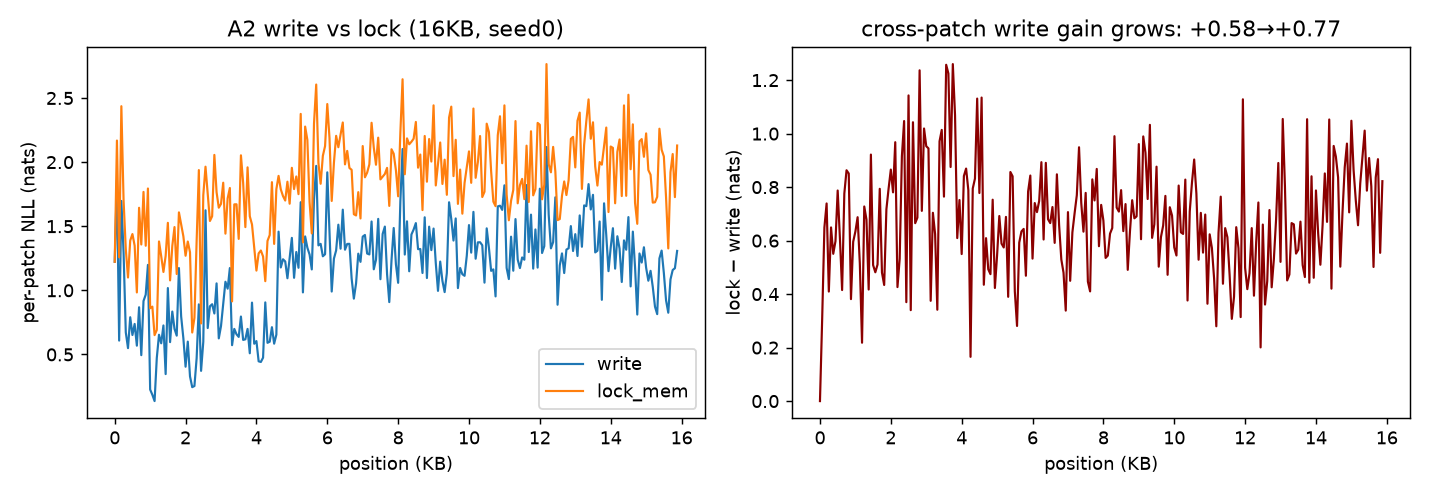
\includegraphics[width=\linewidth]{fig_a2_write_vs_lock.png}
\caption{A2：写入 vs 只读（16\,KB，seed 0）。左：逐 patch NLL；右：$\mathit{lock}-\mathrm{write}$ 的差值，
随上下文增长而增大（前段 $+0.58\to$ 后段 $+0.77$ nats），即跨 patch 写入的收益在累积。}
\label{fig:a2}
\end{figure}

\textbf{判定。}S1 的第二条成立：跨 patch 写入对预测有稳定、可累积的正贡献。
\textbf{注意语义}：$\mathit{lock}$ 只冻结\textbf{跨 patch 的持久写入}，
patch 内的动态通道（$v_{\mathrm{dyn}}$ 与因果分数）仍在工作（表 \ref{tab:surgery}），
所以该对照隔离的是「跨 patch 写入」，不是「全部记忆效应」；
把这一收益拆到具体分量，见 \S\ref{sec:s1-attr}。

\subsection{跨文档边界的信息延续（A3）}\label{sec:a3}

\textbf{设计。}16 篇文档 $\times$ 3072\,B（共 768 个 patch、15 个边界）拼成一条流，
条件：
\textbf{continuous}（状态连续跨文档，即训练时的行为）、
\textbf{reset\_full}（每个边界把状态重置回热启动全态）、
以及重置单个分量的三个变体（在 \S\ref{sec:s1-attr} 中报告）。
指标：整体 bits/byte、边界后 2 个 patch 相对边界前基线的冲击（nats）、
以及回落到「基线 $+0.5\nats$ 以内」所需 patch 数（恢复长度）。

\textbf{结果（表 \ref{tab:a3}、图 \ref{fig:a3}）。}
连续 $1.1032$ 对全重置 $1.1281\bits$；后 14 篇（跳过前 2 篇 burn-in）的平均 NLL：
连续 $0.7711$ 对全重置 $0.7903\nats$，跨文档增益 $-\mathbf{0.0192}\nats$。
边界冲击 $+\mathbf{0.4504}\nats$，恢复长度\textbf{中位数 1 个 patch、最大 2 个 patch}（$n=15$ 个边界）。

% A3 + A5：文档边界与单组件重置
\begin{table}[t]
\centering
\caption{A3 跨文档边界（16 篇文档 $\times$ 3072\,B $=$ 768 patch、15 个边界）与 A5 单组件重置。
冲击 $=$ 边界后 2 个 patch 的平均 NLL 相对边界前 8 个 patch 基线的增量；
恢复长度 $=$ 回落到「基线 $+0.5$\,nats」以内所需的 patch 数。
连续条件无重置点，故不给冲击/恢复。}
\label{tab:a3}
\small
\begin{tabular}{@{}lcccc@{}}
\toprule
条件 & bits/byte & 后段 NLL (nats) & 边界冲击 (nats) & 恢复（中位 / 最大） \\
\midrule
continuous（不重置） & $1.1032$ & $0.7711$ & --- & --- \\
reset\_full（全部重置） & $1.1281$ & $0.7903$ & $+0.4504$ & $1 / 2$ \\
reset \texttt{recurrent} & $1.1241$ & $0.7875$ & $+0.3779$ & $1 / 2$ \\
reset \texttt{memory} & $1.1029$ & $0.7709$ & $+0.0246$ & $0 / 1$ \\
reset \texttt{queue}$+$\texttt{MTM} & $1.1026$ & $0.7708$ & $+0.0250$ & $0 / 1$ \\
\midrule
\multicolumn{5}{@{}l}{跨文档增益（continuous $-$ reset\_full，后 14 篇）：$-0.0192$\,nats；
\ \ \texttt{recurrent} 解释边界冲击的 $84\%$} \\
\bottomrule
\end{tabular}
\end{table}


\begin{figure}[H]
\centering
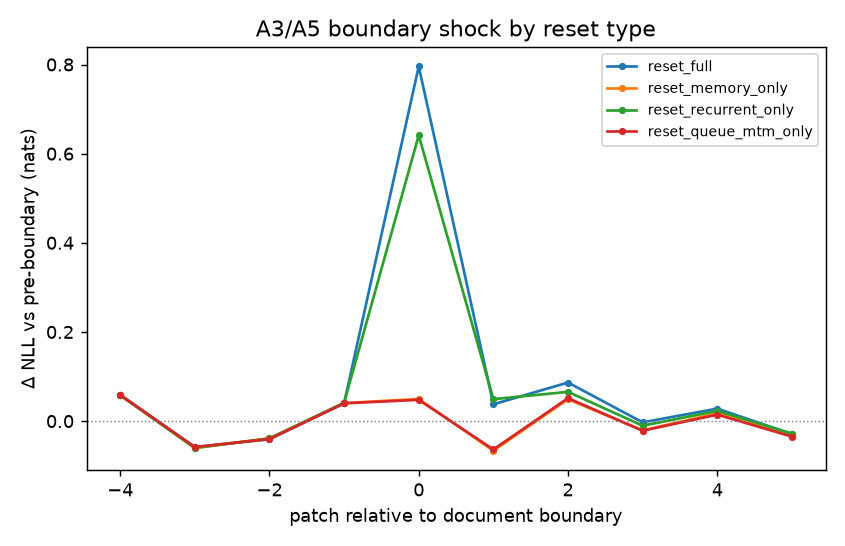
\includegraphics[width=\linewidth]{fig_a3_boundary_recovery.png}
\caption{A3/A5：以文档边界为原点对齐的平均恢复曲线（16 篇文档、15 个边界）。
全部重置的冲击明显；单组件重置的曲线给出归因——\texttt{recurrent} 的曲线几乎复现全重置冲击，
\texttt{memory} 与 \texttt{queue+MTM} 的重置几乎免费。}
\label{fig:a3}
\end{figure}

\textbf{判定。}跨文档的信息延续\textbf{真实但量级小}（$\sim0.02\nats$）；
而边界冲击虽然尖锐（$+0.45\nats$，约合热启动整体水平的量级），却\textbf{在 1--2 个 patch 内自愈}。
这两条合起来说明：固定状态确实把前一篇文章的某种统计结构带进了后一篇，
但「跨文档迁移」不是本文这个检查点的主要收益来源。

\subsection{状态的上下文特异性：错配实验（A4）}\label{sec:a4}

\textbf{设计（未完成）}：用上下文 $A$ 跑出状态，直接在上下文 $B$ 的文档上评测（状态—文本错配），
对照空白态与匹配态；同主题与跨主题各一组，得到 $3\times2$ 的对照矩阵。
\textbf{判读}：错配 $\le$ 空白 $\Rightarrow$ 状态是通用缓存；错配明显更差 $\Rightarrow$ 状态有上下文特异性。
\pending{该实验尚未运行：需要成对主题数据（同主题/跨主题各若干对），
计划与 D 线（\S\ref{sec:dline}）合并成「状态里装的是什么」一节。}
本文目前只用 D 线间接回答该问题（\S\ref{sec:dline}）。

\subsection{组件级归因（A5 / A6）}\label{sec:s1-attr}

\textbf{设计（两种互补的干预）。}
\textbf{A5 重置}：在文档边界处只重置\textbf{一个}分量（\texttt{memory} 回训练稳态快照 /
\texttt{recurrent} 清零 / \texttt{queue+MTM} 清零），其余保持连续；
\textbf{A6 冻结}：在同一份 16\,KB 同分布文本上，每个 patch 前向后把\textbf{一个}分量恢复为前值
（该分量跨 patch 不再更新，patch 内照常更新），与「冻结全部写入」的 $\mathit{lock}$ 及
「全部正常写入」的 write 对照。两者一个问「重置它损失多少」，一个问「冻结它损失多少」。

\textbf{结果（表 \ref{tab:attr}）。}
A5：边界冲击 $+0.3779\nats$（只看 \texttt{recurrent}）对 $+0.4504\nats$（全重置），
即\textbf{84\% 的边界冲击由 \texttt{recurrent} 清零解释}；
只重置 \texttt{memory} 或 \texttt{queue+MTM} 的冲击都是 $\approx+0.025\nats$（近乎免费）。
A6：以 write 为基线，$\mathit{lock}$ 全部写入 $+1.034\bits$，
\textbf{冻结 \texttt{recurrent} $+1.022\bits$}（$\approx$ 全锁的 $98.8\%$，两个 seed 分别 $+0.960/+1.084$），
冻结 \texttt{memory} $-0.0005\bits$，冻结 \texttt{queue+MTM} $+0.0002\bits$——
\emph{都在噪声水平}。

% A6 + B2-freeze：组件归因
\begin{table}[t]
\centering
\caption{组件级归因：两种互补干预在同一份同分布文本上的结果。
（a）A6 冻结（16\,KB，seed $\in\{0,1\}$）：基线为全部正常写入；
（b）B2-freeze（96\,KB，单条流）在自然重复任务上的 $<\!1$k 桶复现增益。
两组的结论一致：代价几乎全部落在 \texttt{recurrent} 上，矩阵记忆与队列 $+$ MTM 无损失。}
\label{tab:attr}
\small
\begin{tabular}{@{}lcc@{}}
\toprule
\multicolumn{3}{@{}l}{\textbf{(a) A6 冻结单分量（16\,KB，2 seed）}} \\
\midrule
条件 & bits/byte（均值） & $\Delta$ vs 全部写入 \\
\midrule
write（全部写入，基线） & $1.386$ & $0$ \\
lock（冻结全部写入） & $2.420$ & $+1.034$ \\
freeze \texttt{recurrent} & $2.408$ & $\mathbf{+1.022}$ \\
freeze \texttt{memory} & $1.386$ & $-0.0005$ \\
freeze \texttt{queue}$+$\texttt{MTM} & $1.386$ & $+0.0002$ \\
\midrule
\multicolumn{3}{@{}l}{\textbf{(b) B2-freeze：自然重复的 $<\!1$k 桶复现增益（nats，96\,KB）}} \\
\midrule
条件 & bits/byte & $<\!1$k 桶增益 \\
\midrule
write & $1.0838$ & $+0.0839$ \\
lock（全程只读） & $2.1641$ & $-0.0050$ \\
freeze \texttt{recurrent} & $2.1527$ & $\mathbf{-0.0043}$ \\
freeze \texttt{memory} & $1.0836$ & $+0.0840$ \\
freeze \texttt{queue}$+$\texttt{MTM} & $1.0832$ & $+0.0837$ \\
\bottomrule
\end{tabular}
\end{table}


\begin{figure}[t]
\centering
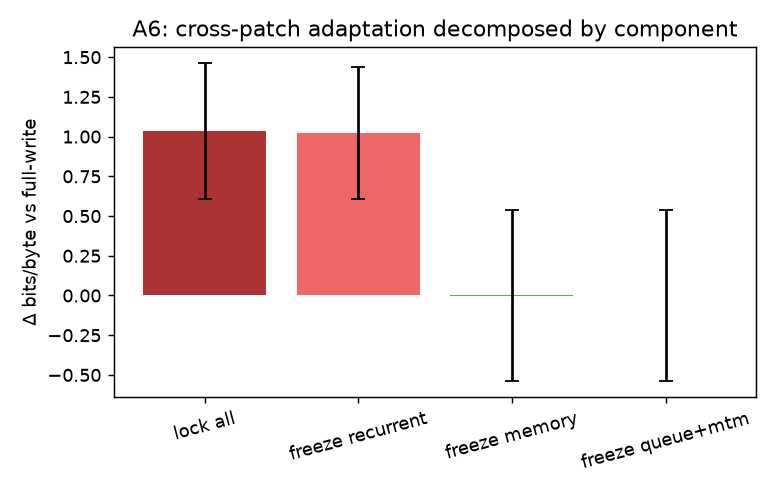
\includegraphics[width=\linewidth]{fig_a6_component_freeze.png}
\caption{A6：跨 patch 适应按组件分解（16\,KB，2 个 seed，误差棒为 95\% CI）。
冻结 \texttt{recurrent} 的代价与冻结全部写入几乎相同；冻结矩阵记忆与队列 $+$ MTM 的代价为零。}
\label{fig:a6}
\end{figure}

\textbf{判定（本文最强的一条归因结论）。}自然文本上的跨 patch 适应\textbf{几乎全部由
\texttt{recurrent}（块级循环状态 \texttt{c\_state}）承担}——
A2（全锁 $+1.00\bits$）、A6（冻结 \texttt{recurrent} $+1.02\bits\approx$ 全锁 $+1.03\bits$）、
A5（边界冲击 $+0.38/0.45\nats$）三个独立实验交叉一致，$4$ 个数量级的不同干预给出同一个答案。
\textbf{这修正了「memory 管长期」的朴素假设}：矩阵记忆在 3\,KB--16\,KB 尺度上是
「一个 patch 即可重建」的快权重，它的价值不在增量适应——冻结其写入几乎零代价，
但它\textbf{读取训练先验}的贡献巨大（去掉热启动后损失升高 $3.7\bits$ 以上，\S\ref{sec:a1}）。
B2-freeze（\S\ref{sec:b2}）在长程复现任务上给出同一归属结论。
\draftnote{版本注：以上归因在 v\_0d3 检查点上测得，其时 \texttt{memory} 跨流共享；
v\_0d4 将其改为序列级私有槽位（\S\ref{sec:model}），「重置 \texttt{memory} $=$ 换共享快照」
的干预语义随之变为「换单流快照」，换用 v\_0d4 检查点后该结论需重新验证。}

\subsection{小结：S1 成立}\label{sec:s1-summary}

\emph{S1 成立}：热启动显著优于空白（$3.73\bits$，同窗口、无收敛趋势），
正常写入显著优于 $\mathit{lock}$（$+1.00\pm0.09\bits$，且随长度累积），两条成立条件同时满足。
归因层面：跨 patch 的信息传递与适应主要由 \texttt{recurrent} 承载，
\texttt{memory} 的作用是\textbf{读取训练稳态先验}，\texttt{queue+MTM} 在本文的尺度上未显示出可测贡献。
